\chapter{Operações Unitárias 1}
\section{Bombas}

Se faz vital o estudo e analise de bombas, principalmente quanto a seu dimensionamento e analise de
rendimento. É claro que necessariamente precisamos dimensionar corretamente o tamanho da bomba, pois
se fazer uma que é excessivamente grande é simplesmente uma perca de dinheiro e energia e uma que
seja menor não sera util para nos. Então esse estudo se faz necessário. Não me destrincharei sobre
os tipos de bombas e suas funcionalidades até por que tem na apostila e nem mesmo a professora foi
tanto nesse aspecto teórico. Então caso tenha interesse, dê uma olhada na apostila. \par

Pois bem, para começarmos nosso estudo, iremos nos virar para a conhecida equação de Bernoulli, dada
por: 
\begin{equation}\label{eq:Eq de Bernoulli}
    \frac{\upsilon ^{2}}{2}+gz_1+\frac{P_1}{\rho }=cte
\end{equation}

Onde \(v_1^{2} \) é a velocidade do liquido, \(g\) é a aceleração da gravidade, \(z_1\) é a altura
do liquido, \(P_1\) é a pressão e \(\rho \) é sua densidade. Inicialmente, vamos fazer algumas
modificações. Para nossas aplicações podemos coloca-la como
\begin{align}\label{eq: EQ das bombas inc}
    \frac{\Delta  \upsilon _ 1^{2}}{2\alpha_{k}}+g \Delta  z+\frac{\Delta  P}{\rho_{1} }+\epsilon =\frac{W_e}{kg} \\
    \alpha_k= \notag
    \begin{dcases}
        0.5, &\text{ se } R_e<2100 ;\\
        1, &\text{ se } R_e>4100 ;\\
    \end{dcases}
\end{align}
onde \(\epsilon \) são as perdas durante o transporte, em principal pelo atrito, \(W_e\) é o
trabalho por unidade de massa, \(R_e\) é o número de Reynolds que diz se nosso escoamento é laminar
ou turbulento. Sua formula é dada por 
\begin{equation}\label{eq:Num de Reynolds}
    R_e=\frac{\rho \upsilon D}{\mu }    
\end{equation}
Vamos fazer uma analise dimensional da nossa equação
\begin{align}
    \frac{\upsilon^{2}}{2\alpha_{k}}&=[\frac{m^{2} }{s ^{2} }]\\
    &=[\frac{m^{2} }{s ^{2} }][\frac{kg}{kg}]\\
    &=[(\frac{mkg}{s ^{2}})][\frac{m}{kg}]\\
    &=[(\frac{Nm}{1})][\frac{1}{kg}]\\
    &=[\frac{J}{kg}]
\end{align}
\begin{align}
    gz_1&=[\frac{m}{s^{2} }][m]\\
    &=[\frac{m^{2} }{s ^{2} }]
\end{align}
O desenvolvimento é o mesmo da velocidade
\begin{align}
    \frac{P_1}{\rho }&=[\frac{Pa}{kg/m^{3}}]\\
    &=[Pa\frac{m^{3}}{kg}]\\
    &=[\frac{N}{m^{2} }][\frac{m^{3}}{kg}]\\
    &=[\frac{Nm}{1}][\frac{1}{kg}]\\
    &=[\frac{J}{kg}]
\end{align}
Vamos fazer uma divisão por g e ver a unidade que nos resta. Como todo sistema tem a mesma unidade,
irei fazer apenas uma vez
\begin{align}
    gz_1&=[\frac{J}{kg}]\\
    &=[\frac{m^{2} kg}{kgs^{2}}]\\
    &=[\frac{m^{2} }{s ^{2} }] [(\frac{1}{m/s ^{2}})]\\
    &=[\frac{m^{2} s ^{2} }{s ^{2} m}]\\
    z_1&=[m]
\end{align}
Logo, teremos apenas unidade de metros. Portanto, \refeq{eq: EQ das bombas inc} fica:
\begin{equation}\label{eq:Eq das bombas}
    \frac{\Delta  \upsilon^{2}}{2\alpha_{k}g}+\Delta  z+\frac{\Delta  P}{\rho_{n}g }+\frac{\epsilon}{g} =\frac{W_e}{g}
\end{equation}
Onde o termo \(\frac{W_e}{g}\) é referenciado como a altura de projeto e geralmente é o que buscamos
e é pedido.\par

Uma ressalva importante, em exercícios, geralmente a pressão dos tanques é igual, a não ser quando
se bombeia o liquido para a parte de baixo de um tanque que está parcialmente cheio, ai temos o peso
da coluna de liquido. Ademais, a parte antes da bomba é chamada de sucção e a posterior é chamada de
recalque. Para considerarmos as alturas, é boa pratica, mas não obrigatório, colocar seu referencial
no centro da bomba.

\subsection{Relação entre \(H_p\) e Vazão}

Como ja temos como calcular a altura de projeto, precisamos relaciona-la com algum aplicação real,
ou seja, precisamos utilizar esse valor para que seja feito o dimensionamento e o calculo de
potencia da bomba. Vamos relacionar, agora, a Altura de projeto \(H_p\) com a vazão volumétrica
\(\dot{\varphi}\). Simplificando \eqref{eq:Eq das bombas} para depender apenas de \(\epsilon\) e
expandindo esse termo
\begin{align}\label{eq:vazao e hp}
    H_p&=\frac{\epsilon_f}{g}\\
    &=\frac{2f}{g}\frac{L+\sum_iL_{eq}}{D}\frac{\overline{\upsilon}^2}{2}\\
    &=\frac{2f}{g}\frac{L+\sum_iL_{eq}}{D}\frac{\dot{\varphi}}{(\pi D^2/4)^2}
\end{align}
Onde \(f\) é o fator de atrito de fanning, sem dimensão. \(L\) é o comprimento do tubo e \(D\) seu
diâmetro. Para um sistema com acréscimo de energia potencial, nossa equação fica
\begin{equation}
    H_p=\Delta z + \frac{2f}{g}\frac{L+\sum_iL_{eq}}{D}\frac{\dot{\varphi}}{(\pi D^2/4)^2}
\end{equation}
Para estimarmos \(f\) vamos usar um diagrama, chamado Diagrama de Moody, onde ele é simples, fácil,
pratico e bastante preciso. Seu gráfico é dado \(f \; vs \; R_e \; vs \; \\ \text{rugosidade
relativa}\). Onde a rugosidade relativa é dado por \(\varepsilon/D\). Podemos usar o diagrama de
Darcy, a única diferença é que o de Darcy é 4 vezes o valor do de Fanny. Vamos falar do \(L_{eq}\)
Ele é equivalente a perda de carga relativa ao acessório. Ela é fornecida pelos fabricantes Ela pode
vir de forma direta, ou pode vir na forma \(L/D\), onde podemos so pegar e multiplicar por \(D\)
para acharmos nosso \(L_eq\). \par
\begin{figure}[H]
    \centering
    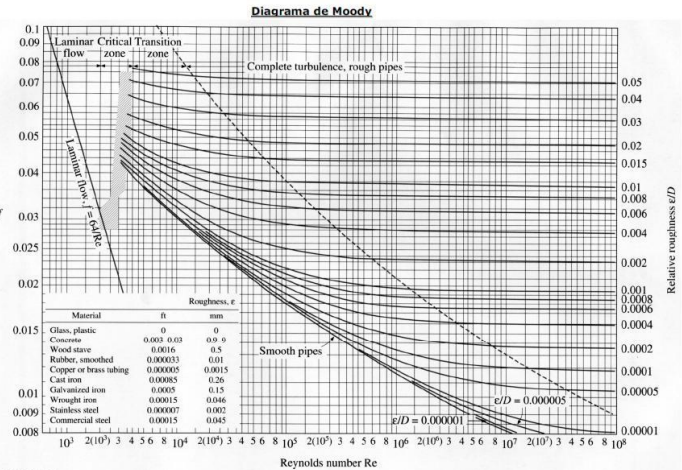
\includegraphics[width=0.8\textwidth]{Diagrama de moody.jpg}
    \caption{Diagrama de Moody}
    \label{fig: diagrama de moody}
\end{figure}    
\subsection{Método dos comprimentos equivalentes}
Esse método consiste em adicionarmos os comprimentos reais dos tubos retos de mesmo diâmetro e os
comprimentos equivalentes \(L_{eq} \) com mesmo diâmetro do conduto, que provocariam a mesma perda
de carga, ou seja, se tivermos um joelho, por exemplo, iriamos considerar o comprimento equivalente
de um tudo de seção reta de mesmo diâmetro que o joelho que causaria a mesma perda de carga. A perda
de carga total, será a soma das perdas de cargas equivalentes, mais as perdas de cargas real da
tubulação. \par Para acharmos o nosso \(L_{eq}\) será nos fornecido uma tabela, o fabricante dará,
de acordo com o material do acessório, que vai nos dar o \(L_{eq}\) para cada acessório e para
vários diâmetros. Em geral, se da as tabelas \(\frac{L}{D}\) pois é mais prático, apenas
necessitando multiplicar pelo \(D\) para obtermos o \(L_{eq} \)
\begin{figure}[H]
    \centering
    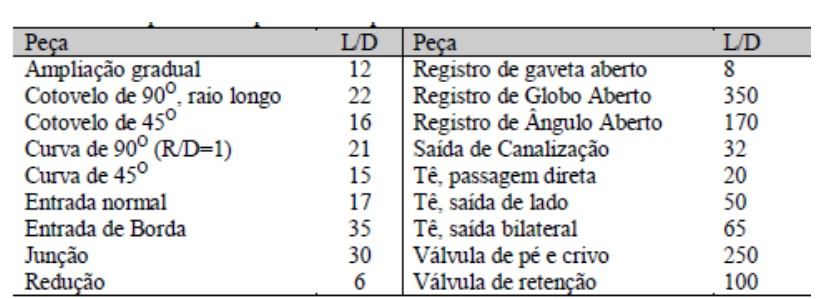
\includegraphics[width=0.8\textwidth]{perdas_equiv.jpg}
    \caption{Perdas equivalentes para diversos acessórios}
    \label{fig: perdas_equiv}
\end{figure}
Caso não tenhamos, sempre podemos utilizar a formula de perda localizada por meio do \(k_f\), ou
seja,
\begin{equation}
    (E_f)_{total} = \left( \frac{4fL}{D} + \sum_{i} k_{f_i} \right) + \frac{\overline{\upsilon } ^{2} }{2} 
\end{equation}
\subsubsection{Exemplos}
Ex1: Se tivermos água a \(20  C^\circ, \rho=1000kgm^{3},\mu=1mPa\cdot s\), é bombeada em estado
estacionário entre 2 reservatórios de alturas iguais. \(P_1=P_2=P_{atm}\). A tubulação tem
\(\varepsilon=0,046 \cdot 10^ {-3}, D=26,6 mm\). A soma de todos os comprimentos retos nos da
\(23,5m\). Considerando 3 curvas de \(90 ^{\circ}\). Ache a cuva de \(\dot{\varphi}\) de \(20-50m^3
h^{-1}\)
\begin{align}
    \intertext{Vamos precisar calcular \(\overline{\upsilon}\) para todos os \(\dot{\varphi}\)}\notag\\.
    \overline{\upsilon}&=\frac{\dot{\varphi}}{(\pi D/4)^2}\\
    \intertext{vamos fazer apenas para \(\dot{\varphi}=20\)}\notag\\
    &=10 m/s\\
    N_re&=\frac{\rho\overline{\upsilon}D}{\mu}\\
    &=2.7\cdot10^5\\
    \frac{\varepsilon}{D}&=\frac{0.046}{26.6}=0.0017\\
    \intertext{Pela analise do grafico \(f=0.0055\)}\notag\\
    \intertext{Eles nos disse que \(L_{eq}=\)3 cantos de 90, olhando na tabela, teremos \(L_{eq}=0.396 m\)}\notag\\
    \intertext{Substituindo em \eqref{eq:vazao e hp}}\notag\\H
    H_p&=\frac{2 \cdot 0.0055}{9.81}\frac{23.5+3(0.396)}{0.0266}\frac{\dot{\varphi}^2}{\pi (0.0266)^2/4}\\
    &=3.37 \cdot 10^6 \dot{\varphi}^2\\
    &=3.37 \cdot 10^6 0.0056 m^3/s\\
    &=114.38 m
\end{align}
\begin{figure}[H]
    \centering
    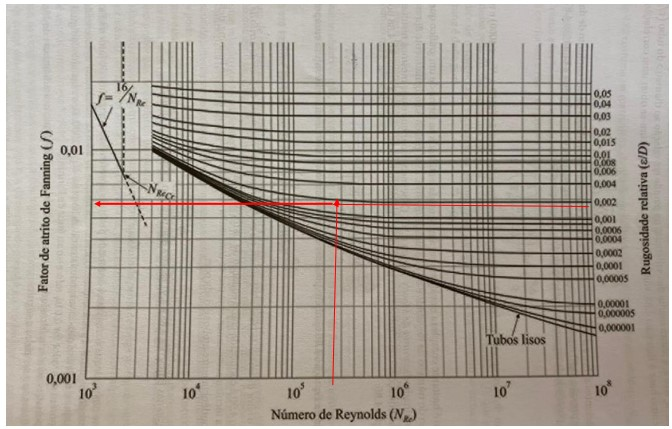
\includegraphics[width=0.8\textwidth]{diagrama_moody_ex.jpg}
    \caption{Diagrama de moody para o exemplo}
    \label{fig: diagrama_moody_ex}
\end{figure}
\begin{figure}[H]
    \centering
    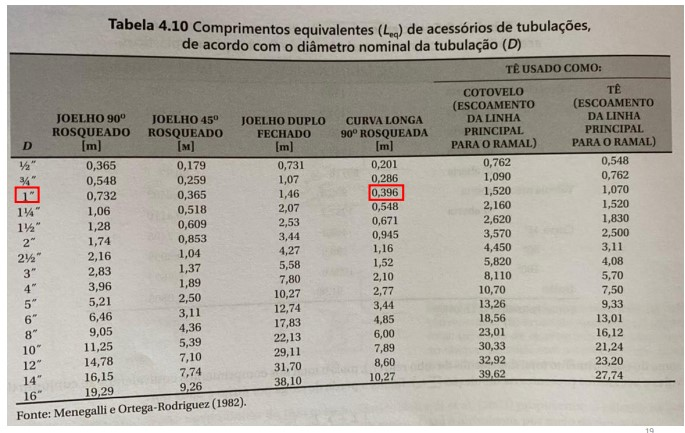
\includegraphics[width=0.8\textwidth]{leq_exemplo.jpg}
    \caption{Comprimentos equivalentes para o exemplo}
    \label{fig: leq_exemplo}
\end{figure}
Como temos \(H_p(\dot{\varphi})\), podemos traçar a curva característica da bomba, onde
posteriormente podemos cruzar com a bomba do fabricante e podemos dimensionar nossa bomba.
\begin{figure}[H]
    \centering
    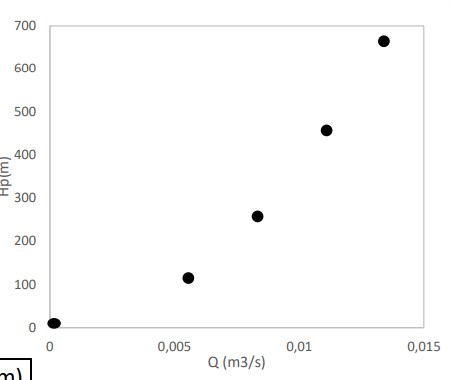
\includegraphics[width=0.8\textwidth]{curva_da_bomba.jpg}
    \caption{Curva característica da bomba}
    \label{fig:curva_da_bomba}
\end{figure}

Ex2: Considere o exemplo em que água a \(20^{\circ }, \rho = 1000 \frac{kg}{m^3}, \mu = 1 mPa s\) é
bombeada a uma diferença de altura de \(20 m\). Considere que o nível da água em cada um dos tanques
é mantido constante ao longo do tempo e que ambos reservatórios são abertos para atmosfera. A
tubulação é de aço comercial tem diâmetro interno constante de \(26,6 mm\)  (Sch. 40, diâmetro
nominal 1”) e a soma do comprimento de todos os trechos de tubo reto resulta em 42 m. Para calcular
as perdas de energia, considere 4 curvas longas de \(90^{\circ } \)  rosqueadas e despreze as perdas
devidas à entrada e saída do fluido na tubulação. Construa a curva da variação da altura de projeto
em função da vazão volumétrica na faixa de \(1-50\) 
\begin{align}
    L &= 42 m\\
    D &= 26.6 \cdot 10^{-3} \\
    R_e = \frac{\rho \overline{\upsilon} D}{\mu} &= 1000 \cdot \frac{6.94 \cdot 10^{-3}}{(\pi (26.6 \cdot 10^{-3})^2/4)^{2} } \cdot 26.6 \cdot 10^{-3} 
    \frac{\varepsilon}{D} &= \frac{0.046}{26.6} = 0.0017\\
    f &= 0.0055\\
    L_{eq} &= 4 \cdot 0.396 = 1.584 m\\
    H_p &= \frac{2f}{g} \frac{L + \sum_i L_{eq}}{D} \frac{\dot{\varphi}^2}{(\pi D^2/4)^2} + 20\\
    H_p &= \frac{2 \cdot 0.0055}{9.81} \frac{42 + 1.584}{26.6 \cdot 10^{-3} } \frac{\dot{\varphi}^2}{(\pi (26.6 \cdot 10^{-3})^2/4)^2} + 20\\
    H_p &= 60 \cdot 10^5 \dot{\varphi}^{2} + 20\\
    \intertext{Com \(\varphi  = 2.78 \cdot 10^{-3} \) }\\
    H_p &= 66.3704 m
\end{align}

%────────────────────────────────────────────────────────────────────────────────────────────────────────────────────────────────────────────────────
% Ex3: Considere a instalação representada na Figura 3, para transportar \(\varphi = 25
% \frac{m^{3}}{h} \)  de etanol a 25oC (\(\mu = 1.10 \cdot 10-3 Pa.s\) ; \(\rho  = 788 Kg/m^3\) ;
% \(P_v = 7,83 kPa\) ). A tubulação é de aço comercial com a tubulação da sucção com diâmetro
% interno de \(77,9 mm\)  (diâmetro nominal 3”, Sch. 40), e a de recalque com diâmetro interno de
% \(62,7 mm\)  (diâmetro nominal 21/2”, Sch. 40). Em todas as mudanças de direção curvas longas
% (cotovelos) de \(90^{\circ } C\)  estão instaladas. \begin{align} L &= 7 m D_{suc}  &= 77.9 \cdot
% 10^{-3} \\
%     D_{rec} &= 62.7 \cdot 10^{-3} \\
%     \varphi &=  \frac{25}{3600} = 6.94 \cdot 10^{-3} m^3/s\\
%     R_{e_{suc} } &= \frac{\rho \overline{\upsilon} D_{suc} }{\mu} = \frac{(788)(\frac{6.94 \cdot
%     10^{-3}}{(\pi (77.9 \cdot 10^{-3})^2/4)})(77.9 \cdot 10^{-3})}{1.10 \cdot 10^{-3}} = 81.3
%     \cdot 10^{3}\\
%     R_{e_{suc}} &= \frac{\rho \overline{\upsilon} D_{rec} }{\mu} = \frac{(788)(\frac{6.94 \cdot
%     10^{-3}}{(\pi (62.7 \cdot 10^{-3})^2/4)})(62.7 \cdot 10^{-3})}{1.10 \cdot 10^{-3}} = 101.061
%     \cdot 10^{3}\\
%     \frac{\varepsilon}{D_{suc} } &= \frac{0.046 \cdot 10^{-3}}{77.9 \cdot 10^{-3}} = 0.000591\\
%     f_{suc} &= 0.021\\
%     f_{rec} &= 0.023\\
%     \intertext{A perda de carga a na sucçao é dada por} \notag\\
%     H_{p_{suc} } = 2 \cdot f_f \cdot \frac{L_{eq} }{D} \upsilon^{2} = 2 \cdot 5.25 \cdot 10^{-3}
%     \cdot \frac{15.9}{77.9 \cdot 10^{-3}} \cdot \frac{(6.94 \cdot 10^{-3})^{2}  }{(\pi (77 \cdot
%     10^{-3})^{2}/4)^{2}} = 4.76 / 9.81 = 0.485 m \intertext{A perda de carga a na recalque é dada
%     por} \notag\\
%     H_{p_{rec} } = 2 \cdot f_f \cdot \frac{L_{eq} }{D} \upsilon^{2} = 2 \cdot 5.75 \cdot 10^{-3}
%     \cdot \frac{22.2}{62.7 \cdot 10^{-3}} \cdot \frac{(6.94 \cdot 10^{-3})^{2}  }{(\pi (62.7 \cdot
%     10^{-3})^{2}/4)^{2}} = 20.57 / 9.81 = 2.096 m \intertext{Somando as energias potencias} \notag
%     \\
%     H_{p_{suc} } = 24.058 - 5 = 19.058\\
%     H_{p_{rec} } = 16.77 + 4.5 = 21.27\\
%     H_p = H_{p_{suc} } + H_{p_{rec}} + \frac{\upsilon_2 ^{2} - \upsilon_1 ^{2}}{2g} +
% \frac{P_1}{\rho g} = -19.058 + 21.27 + \frac{2.25^{2} - 1.4569^{2}}{2 \cdot 9.81} + \frac{7.81
% \cdot 10^{3} }{788 * 9.81} \end{align}
% ────────────────────────────────────────────────────────────────────────────────────────────────────────────────────────────────────────────────────
\subsection{Trabalho e Capacidade da Bomba}
Altura desenvolvida pela bomba pode ser definida como o trabalho por unidade de massa do fluido que
a bomba é capaz de fornecer, escoando a determinada vazão, sendo comum ignorar os termos de
\(E_c,E_p\), apenas considerando a pressão, logo
\begin{equation}
    H_p = \frac{P_2 - P_1}{\rho g}
\end{equation}
 \subsubsection{Capacidade da bomba}
 Referenciada por \(\dot{\varphi }\) referencia a quantidade de fluido que a bomba consegue
 descarregar por unidade de tempo. Expressa, normalmente em \(m^3/h, m^3/s, etc\). 
 \subsubsection{Potencia Util}
 Definida como potencia fornecida ao fluido na vazão mássica desejada, sua equação é
 \begin{equation}
     P_{util} = \dot{m}gH_p = \dot{m}W = \rho \dot{\varphi} W_e
 \end{equation}
 A eficiência é dado por
 \begin{equation}
     \eta = \frac{P_{util}}{P_{consumida}}
 \end{equation}
 Para bombas centrifugas a eficiência é chamada de eficiência mecânica \(\eta_{mec}\) e eficiência
 elétrica \(\eta_e\). Portanto a eficiência glocal é dado como
 \begin{equation}
     \eta_{global} = \eta_{mec} \eta_e = \frac{P_{util}}{P_{el}}
 \end{equation}
 Potencia util que a gente vai usar
 \begin{equation}
    P_0 = \frac{\rho \dot{\varphi} H_p}{\eta }
 \end{equation}
 \subsection{Curvas do fabricante}
 A altura \(H_p\) é determinada experimentalmente pelo fabricante, sendo fornecida por meio de uma
 curva que relacionam \(H_p, \dot{Q}, P_e, \eta_{mec}\). A capacidade de uma  bomba é se relaciona
 diretamente com o diâmetro do rotor, de forma que quanto maior o diâmetro, maior a capacidade da
 bomba. \par Quando achamos nossa curva característica da bomba, vamos cruzar cm a curva do
 fabricante, ou seja onde se cruzar as duas curvas é o nosso ponto de operação. Mas onde tem a
 eficiência maxima, nem sempre vai ser onde vai ter o ponto de operação.
 \begin{figure}[H]
    \centering
    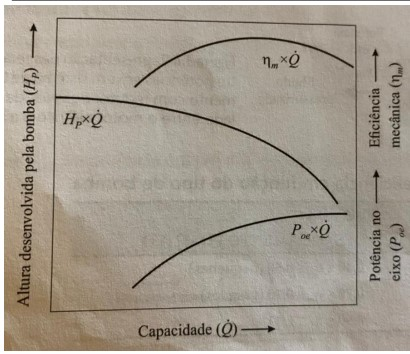
\includegraphics[width=0.8\textwidth]{curva_bomba.jpg}
    \caption{Curva característica das Bombas}
    \label{fig: curva_bomba}
 \end{figure}
 \begin{figure}[H]
    \centering
    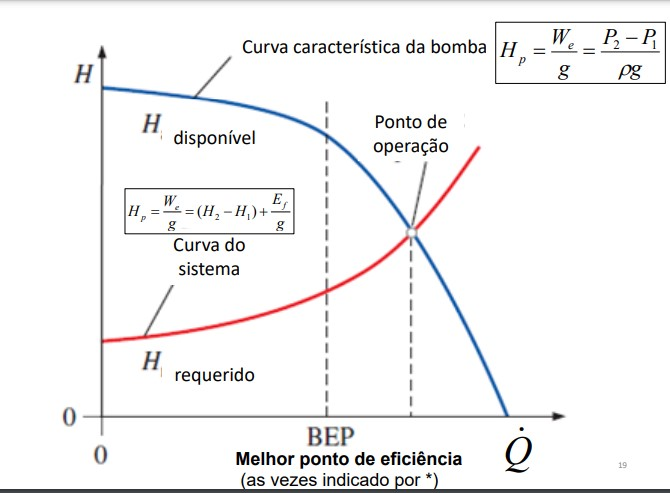
\includegraphics[width=0.8\textwidth]{ponto_operacional.jpg}
    \caption{Ponto de operação de uma bomba}
    \label{fig: ponto_operacional}
 \end{figure}
 \subsection{Curvas de desempenho da bomba}
 Essas curvas vão nos mostrar os melhores desempenhos das bombas e também seu range de operação e
 como sua eficiência varia com essa operação. \par
 
 Alguns pontos importantes são:
    \begin{itemize}
        \item {Ponto de operação: \\
        Ponto onde a bomba opera, ou seja, onde se cruzam as curvas do fabricante e a característica
        da bomba.}
        \item {Ponto de melhor eficiência: \\
        Ponto onde a eficiência é maxima.}
        \item {Ponto de melhor eficiência operacional: \\
        Ponto onde a eficiência é maxima e a vazão é maxima.}
        \item {Ponto de carga de fechamento: \\
        Altura desenvolvida pela bomba quando a carga é zero, ocorrendo quando a saída da bomba é
        bloqueada, não realizando trabalho util}
        \item {Ponto de fornecimento livre: \\
        Ponto onde a bomba opera sem carga, ou seja, quando a vazão é maxima.}
    \end{itemize}
A eficiência maxima é atingida entre o ponto de carga de fechamento e o ponto de fornecimento livre,
no ponto de maxima eficiência
\subsection{Altura de sucção disponível}
Existe um limite inferior no valor de pressão que pode atingir na sucção de uma bomba e caso esse
nível seja atingindo, ocorrera a cavitação, que é a formação de bolhas quando a bomba trabalha
abaixo desse limite. Se a pressão no interior da bomba for inferior a pressão do vapor do liquido na
mesma temperatura pode ocorrer a cavitação. Vai acontecer a vaporização parcial, formando bolhas que
vao estourar dentro da bomba e podem levar a corrosão do motor da bomba, dentre outros problemas.
Para evita-la, podemos estabelecer uma margem de segurança para a pressão de sucção da bomba. Esse
valor é achado por meio de um balanco de energia mecânica. Sua formula é:
\begin{equation}\label{eq: NPSH}
    NPSH = \frac{1}{g}\left( \frac{\Delta P_{succao}}{\rho} + \frac{\Delta \overline{v}^2_{sucç\tilde{a}o}}{2 \alpha _k}\right) - \left(\frac{P_v}{\rho g}\right)
\end{equation}
Para não cavitar nosso valor da bomba tem que ser maior que o \(NPSH\). Se o fluido não for água,
converter em coluna de água. O NPSH da bomba é dado ou ele pode ser achado em uma tabela
\begin{equation}
    NPSH_{bomba} > NPSH_{sistema}  
\end{equation}
Para o \(NPSH\) disponível do sistema, temos o balanço de energia que vai nos dar
\begin{align}
    \frac{P_2 - P_1}{\rho g} + \frac{\overline{\upsilon } ^{2} }{2g} + z_2 - z_1 + \frac{\varepsilon}{g} = 0
    \frac{1}{g} \left( \frac{P_2}{\rho } + \frac{\overline{\upsilon }^{2}_2}{2}  \right) = \frac{P_1}{\rho g} - \Delta z - \frac{\varepsilon}{g}
\end{align}
Nosso balanco é feito desde o começo do reservatório ate a entrada da bomba e nosso valor tem que
ser maior que o achado pela formula \eqref{eq: NPSH}. \(P_v\) é a pressão de vapor do liquido.
\subsection{Escolha da bomba}
A escolha da bomba pode ser feita por meio de um gráfico, onde temos a altura de projeto e a vazão
volumétrica. 
\begin{figure}[H]
    \centering
    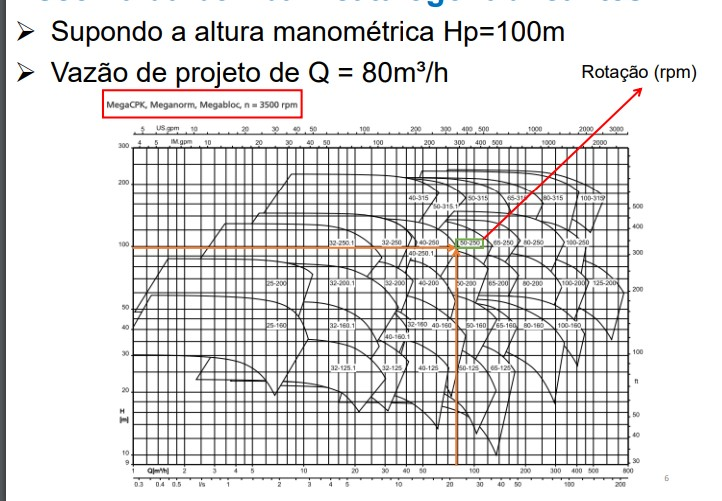
\includegraphics[width=0.8\textwidth]{escolha_bombas.jpg}
    \caption{Gráfico da escolha da bomba}
    \label{fig: escolha_bomba}
\end{figure}
\begin{figure}[H]
    \centering
    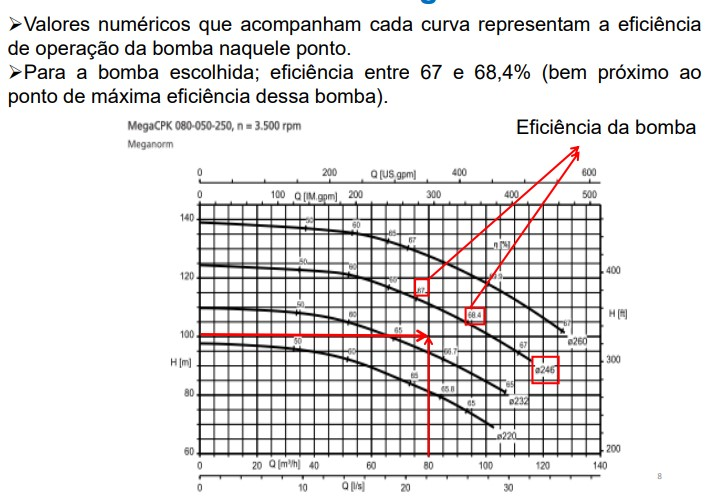
\includegraphics[width=0.8\textwidth]{eficiencia_grafico.jpg}
    \caption{Eficiência da bomba por escolha}
    \label{fig: eficiencia_bom}
\end{figure}
%────────────────────────────────────────────────────────────────────────────────────────────────────────────────────────────────────────────────────

\section{Agitação e mistura}
Uma  das partes mais importantes é a questão da agitação e mistura do nosso liquido. Precisamos
dimensionar bem a potencia e as pas e tamanhos do nosso agitador. Nossa potencia fornecida pelo
motor \(P_o\) sera função de diversas variáveis dentre elas estão a \(\rho\), densidade, \(\mu\)
viscosidade, \(N\) frequência rotacional do impulsor, \(D_a\) diâmetro do agitador \(D_t\) diâmetro
do tanque, \(H_a\) altura do agitador desde a base do tanque, \(H_l\) altura do líquidos, \(w_d\),
largura dos defletores, além do tipo de agitador com sua característica altura das pas \(H_p\),
logo, nossa função é
\begin{align}
    P_o = f(\rho, \mu, N, D_a, D_t, H_a, w_d, g)
\end{align}
Porem, conseguimos reduzir para variáveis adimensionais, com o uso do numero de Reynolds de potencia
e Froude de potencia
\begin{equation}
    N_{P_o} = \frac{P_0}{N^3D_a^5 \rho}
\end{equation}
E o de Froude
\begin{equation}
    N_{fr} = \frac{N^2D_a^2}{g}
\end{equation}
Além disso, definimos mais números adimensionais como 
\begin{equation}
    \frac{D_t}{D_a}, \frac{H_a}{D_a}, \frac{H_L}{D_a}, \frac{w_d}{D_a}
\end{equation}
Logo, nossa função fica
\begin{equation}
    P_0 = f(N_{re}, N_{fr}, \frac{D_t}{D_a}, \frac{H_a}{D_a}, \frac{H_L}{D_a}, \frac{w_d}{D_a})
\end{equation}
Lembrando que \(N_fr\) deve ser considerado quando ha formação de vórtice junto ao eixo, sendo
importante para \(N_{re} > 300\) e para tanques sem defletores.
\subsection{Calculo de Potencia para agitadores Newtonianos}
O caso mais simples sao aqueles que a velocidade angular, tipo de agitador e dimensões geométricas
ja foram definidas previamente. Para esse caso, precisamos calcular apenas a energia dissipada pelo
agitador nessas condições e posteriormente determinar \(N_{P_o}\) As dimensões mais usadas sao
\begin{equation}
    \begin{split}
        \frac{D_t}{D_a} = 3\\
        \frac{H_a}{D_a} = 1\\
        \frac{H_l}{D_a} = 3\\
        \frac{w_d}{D_t} = 0.1\\
        \frac{H_a}{D_t} = \frac{1}{3}\\
        \frac{H_L}{D_t} = 1\\
        \frac{w_d}{D_t} = \frac{1}{12}\\
        \frac{H_p}{D_a} = \frac{1}{5}
    \end{split}
\end{equation}
As curvas de \(N_{p_0} \times N_{re}\) sao determinados experimentalmente para os diferentes tipos
de agitadores. Para a região laminar, (\(N_{re} < 10\)) a relação
\begin{equation}
    N_{P_o} = \frac{K_p}{R_{re}}
\end{equation}
Em que \(K_p\) é uma constante adimensional. Na região de turbulência, \(N_{P_0} = K_p\). Em geral
\(K_p\) tem valores constantes e dependem do agitador, numero de defletores e sua dimensão.

%────────────────────────────────────────────────────────────────────────────────────────────────────────────────────────────────────────────────────

\section{Caracterização de Partículas Solidas}
Um solido particulado pode ser caracterizado como um material composto por partículas de tamanho
muito reduzidos. Vamos definir algumas propriedades importantes. 
\begin{itemize}
    \item {Esfericidade \(\phi\):\\
    Útil para caracterizar a forma de partículas irregulares. Ele  leva a extensão do desvio entre a
    partícula real e a do formato esférico.\\
    \begin{equation}
        \phi = \left\lVert\frac{A_{esfera}}{A_{part \acute{i} cula}}\right\rVert_V \leq 1
    \end{equation}
    \(A_{esfera}\) = área superficial da esfera de igual volume da partícula \(A_{part \acute{i}cula}\) =
    Área superficial da partícula}
    \item {Densidade: \\
        Definida como a razão entre a massa e o volume da partícula.\\
        Como as partículas geralmente tem poros, a densidade pode ser tomada considerando ou nao os
        poros.\\
        Podemos definir como Densidade real (\(\rho_s\)), Densidade da partícula (\(\rho_p\)) e
        Densidade aparente (\(\rho_a\)).\\
        \begin{itemize}
            \item {A densidade real se da como a densidade excluindo os poros.
                \begin{equation}
                    \rho_s=\frac{m_p}{V_{sem poros}}
                \end{equation}
        }
            \item { A densidade da partícula se da como a densidade excluindo poros intersticiais.
                \begin{equation}
                    \rho_p=\frac{m_p}{V_{compactado}}
                \end{equation}
                No fim a real e a aparente sao basicamente iguais. }
            \item { A densidade aparente se da como a densidade incluindo os poros intersticiais.
                \begin{equation}
                    \rho_a=\frac{m_p}{V_{total}}
                \end{equation}
        } \end{itemize}}
        \item {Porosidade: Pode ser separada entre a aparente e a real.\\
            A aparente tem formula
            \begin{equation}
                \varepsilon_{ap} = 1 - \frac{\rho_ap}{\rho_s}
            \end{equation}

        }
        \item { Área superficial especifica:\\
            A area superficial especifica se da como a razão entre a area superficial da partícula e
            o volume da partícula.\\
            \begin{equation}
                a_s=\frac{A_sp}{V_p}
            \end{equation}
            \(A_{sp}\) = Área superficial da partícula\\
            \(V_p\) = Volume da partícula\\
            Para uma esfera vamos ter
            \begin{equation}
                a_s=\frac{6}{D_p}
            \end{equation}
        }     
\end{itemize}
\subsection{Tamanho de partículas}
Para medir o tamanho da partícula é bastante simples, so medir com um paquímetro. Porem, claro,
temos \(n\) partículas. Para uma peneira de Tyler, o diâmetro médio de partículas é dado por
\begin{equation}
    \overline{D} = \frac{1}{\sum_i X_n/\overline{a_n}}
\end{equation}
Em que \(X_n\) é a fração mássica retirada na peneira e \(\overline{a_n}\) é a media entre a
abertura entre duas peneiras. \par Para uma partícula em que a area superficial é igual a medias das
areas superficiais de todas as partículas presentes em uma amostras, temos
\begin{equation}
    \overline{D}_p = \sqrt{\frac{\sum_{n= 1}^j \frac{X_n}{\overline{a}_n}}{\sum_{n= 1}^j \frac{X_n}{\overline{a}_n^3}}}
\end{equation}
Para uma partícula cujo volume é igual ao volume médio de todas as partículas presentes em uma
amostra, temos
\begin{equation}
    \overline{D}_v = \sqrt[3]{\frac{1}{\sum_{n= 1}^j \frac{X_n}{\overline{a}_n^3}}}
\end{equation}
\subsection{Relação entre \(D_{eq}\)  e \(D_p\) }
\begin{enumerate}
    \item {Para partículas irregulares que nao aparentam compridas nem curtas, temos
    \begin{equation}
        D_{eq} = \phi D_{esp} \approx = \phi D_p
    \end{equation}
    }
    \item {Para partículas alongadas, temos
    \begin{equation}
        D_{eq} = \phi D_{esp} \approx =  D_p
    \end{equation}
    }
    \item {Partículas irregulares, mas curtas, temos
    \begin{equation}
        D_{eq} = \phi D_{esp} \approx = \phi^2 D_p
    \end{equation}
    }
\end{enumerate}
\subsection{Distribuição de tamanho de partículas}
A distribuição de tamanho de partículas é uma função que relaciona o tamanho da partícula com a
fração de partículas com aquele tamanho. Vao nos dar uma curva de distribuição de tamanho de
partículas.\\
\subsubsection{Modelos de Distribuição Granulometrica}
As propriedades das partículas dependem de sua granulometria. No mundo real, existem diversas
partículas nao uniformes, sendo necessário conhecer o comportamento do particulado. Se ve muito
importante, em principal, descobrir o diâmetro médio dos particulados, para isso, existem modelo de
distribuição do material, como, por exemplo, o modelo de Gates-Gaudin-Schumann, GGS, dado por
\begin{equation}
    X_f = \left(\frac{a_n}{K_{GGS}}\right)^{IGGS}
\end{equation}
Em que \(X_f\) é a fração mássica do material mais fino do que a abertura da peneira, \(a_n\) é a
abertura da peneira de ordem \(n\). \(K_{GGS}\) é o parâmetro médio das partículas e \(IGGS\) é o
parâmetro que representa a distribuição das partículas.\par

Distribuição de Rosin-Rammler, RR, dada por
\begin{equation}
    X_f = 1 - e^{-\left(\frac{a_n}{K_{RR}}\right)^{I_{RR}}}
\end{equation}
Em que \(K_{RR}\) é o parâmetro médio das partículas e \(I_{RR}\) é o parâmetro que representa a
distribuição das partículas.\par
%Desenhemos um gráfico de distribuição de tamanho de partículas \begin{tikz} \begin{axis}[ axis
% lines = left, xlabel = \(a_n\), ylabel = \(X_f\),
%         ]
%         \addplot [
%             domain=0:10, 
%             samples=100, 
%             color=red,
%             ]
%             {1 - e^(-(x/0.036)^0.2751)};
%         \addlegendentry{RR}
%         \addplot [
%             domain=0:10, 
%             samples=100, 
%             color=blue,
%             ]
%             {(x/0.298)^0.072};
%         \addlegendentry{GGS}
%     \end{axis}
% \end{tikz}

%Continuar depois
%────────────────────────────────────────────────────────────────────────────────────────────────────────────────────────────────────────────────────

\section{Dinâmica de partículas}
Entender essa parte é importante para entender diversas operações unitárias que envolvem partículas.
Essas ideias podem ser implementadas em diversas operações industriais, como a industria do leite em
po,  cafe, etc. \par

Seja uma partícula sobre ação da forca de gravidade, uma forca de arraste e uma forca de empuxo. Se
definirmos a forca como \(F = m \frac{\mathrm{d}v }{\mathrm{d}x }\)  vamos ter que a forca
resultante é dada por
\begin{equation}\label{eq: forca resultante}
    F = m \frac{\mathrm{d}v }{\mathrm{d}t } = F_{ext} - F_a - F_e
\end{equation}
Em que \(F_a\) é a forca de arraste e \(F_e\) é a forca de empuxo. \par A forca externa é dado por 
\begin{equation}\label{eq: forca externa}
    F_{ext} = m a_c
\end{equation}
A forca de arraste é dada por
\begin{equation}\label{eq:forca de arraste}
    F_d = \frac{1}{2} \rho_f C_d A_f v^2
\end{equation}
Em que \(\rho_f\) é a densidade do fluido, \(C_d\) é o coeficiente de arraste, \(A_f\) é a area de
referencia e \(v\) é a velocidade da partícula. \par

A forca de empuxo é dada por
\begin{equation}\label{eq: forca de empuxo}
    F_e = \left( \frac{m}{\rho_p} \right) \rho g
\end{equation}
Em que \(\rho_p\) é a densidade da partícula, \(\rho\) é a densidade do fluido e \(g\) é a
aceleração da gravidade. \par

Voltando ao coeficiente de arraste, ele depende de diversos fatores, dentre eles o numero de
Reynolds, \(Re\), para uma partícula esférica, temos
\begin{equation}
    Re = \frac{\rho_f v D_p}{\mu_f}
\end{equation}
Em que \(\mu_f\) é a viscosidade do fluído e \(D_p\) é o diâmetro da partícula. Para valores de
numero de Reynolds pequenos, a forca de arraste de uma esfera é dada por 
\begin{equation}
    F_d = 3 \pi \mu_f D_p v
\end{equation}
O coeficiente de arrasto predito pela lei de Stokes é dado por, para o regime laminar (\(N_{re} <
0.4 \) ):
\begin{equation}
    C_d = \frac{24}{Re}
\end{equation}
Para o regime de transição (\(0.4 < N_{re} < 500 \) ):
\begin{equation}
    C_d = \frac{10}{\sqrt{R_e}}
\end{equation}
Para o regime turbulento (\(N_{re} > 500\) ) o coeficiente de arraste é  \(0.44\), determinado
experimentalmente. \par 
\subsection{Velocidade Terminal}
Para um partícula caindo sobre ação da gravidade e da forca de arraste, temos 2 estágios dda
velocidade, aquela em  que a velocidade estará aumentando devido a forca da gravidade e aquela a
qual a velocidade se estabiliza e a partícula cai com velocidade constante. Essa velocidade
constante é chamada de velocidade terminal, \(\upsilon _t\). \par 

O período a qual a partícula esta sendo acelerada é bastante curto e a maioria do movimento acontece
sobre o efeito da velocidade terminal. Logo, o tempo gasto para que a queda da partícula é calculado
com base no período de velocidade constante, ou seja, quando nossa aceleração é zero e as forcas se
equivalem. \par

Substituindo nossas expressões das forcas na equação da segunda lei de Newton, ou seja, \eqref{eq:
forca de arraste}, \eqref{eq: forca externa} e \eqref{eq: forca de empuxo} em \eqref{eq: resultade
forcas} temos
\begin{align}
    \frac{\mathrm{d}\upsilon }{\mathrm{d}t} &= g \left( 1 - \frac{\rho}{\rho _{p} }  \right) - \left( \frac{C_{d} \upsilon ^{2} \rho A_{p} }{2m} \right)\\
    &= g \left( 1 - \frac{\rho}{\rho _{p} }  \right) - \left( \frac{C_{d} \upsilon ^{2} \rho \pi D_{p}^{2} }{8m} \right)\\ 
\end{align}
Assumindo que a partícula esta em velocidade terminal, ou seja, \(\frac{\mathrm{d}\upsilon
}{\mathrm{d}t} = 0\) e que a partícula seja esférica, com \(A_{p} = \frac{\pi D_{p} ^{2} }{4}\) e
\(\rho _{p} = \frac{6m}{\pi D_{p} ^{3} }\), vamos ter
\begin{equation}
    \frac{3C_{d} \upsilon _{t} ^{2} \rho }{4D_{p}\rho _{p}  }  = g \left( 1 - \frac{\rho}{\rho _{p} }  \right)
\end{equation}  
Isolando a velocidade terminal, temos
\begin{equation}
    \upsilon _{t} = \sqrt{\frac{4gD_{p}\left( \rho _{p} - \rho \right) }{3C_{d} \rho }  }
\end{equation}
Essa expressão é valida para qualquer regime de escoamento. Conseguimos fazer algumas distinções
para alguns casos, dado o numero de Reynolds e a geometria da partícula. \par
\subsubsection{Primeiro Caso}
Escoamento lento, ou seja, \(N_{re} < 0.4\), para uma partícula esférica, temos
\begin{equation}
    \upsilon _{t} = \frac{\left( \rho _{p} -\rho  \right) g D_{p} ^{2} }{18\mu }
\end{equation}
\subsubsection{Segundo Caso}
Para região intermediaria, ou seja, regime de transição \(0.4 < N_{re} < 500\), temos
\begin{equation}
    \upsilon _{t} = \left(\frac{4\left( \rho _{p} -\rho  \right)^{2} g^{2}}{225 \rho \mu ^{2} } \right)^{\frac{1}{3}}D_{p} 
\end{equation}
\subsubsection{Terceiro Caso}
Para regime turbulento, ou seja, \(N_{re} > 500\), temos que \(C_{d} =0.44\), logo:
\begin{equation}
    \upsilon _{t} = \sqrt{\frac{3.03\left( \rho _{p} -\rho  \right) gD_{p}}{\rho }  }
\end{equation}
%────────────────────────────────────────────────────────────────────────────────────────────────────────────────────────────────────────────────────
\section{Leitos Porosos}
Leitos porosos são amplamente utilizados em processos de separação, como por exemplo, na secagem de
grãos, na filtração de água, na adsorção de gases e líquidos, na remoção de partículas de um fluido,
etc. \par

A depender de como o solido esta se movimentando no leito, podemos ter 2 tipos de leitos
\begin{itemize}
    \item Leito Fixo: O solido esta parado e o fluido esta se movimentando
    \item Leito Móvel: A velocidade do fluido é suficiente para provocar movimentos aleatórios nas
    partículas do leito
\end{itemize}
\subsection{Propriedades físicas do leito}
Os leitos sao caracterizados pela granulometria das partículas, area especifica, porosidade e
densidade. Para as partículas em conjunto, podemos ter um leito fixo, fluidizado ou nevoa. \par
\subsubsection{Densidade global do leito}
A densidade global do leito é quando o material esta empacotado ou empilhado, sendo definido como a
razão entre a massa do material e o volume que ele ocupa. Matematicamente, temos
\begin{equation}
    \rho _{b} = \frac{m_{p} + m_{fluid} }{V_{L} } = \frac{m_{p} + m_{fluido}}{V_{s} + V_{v} }
\end{equation}
Onde \(m_{p}\) é a massa das partículas, \(m_{fluid}\) é a massa do fluido, \(V_{L}\) é o volume do
leito, \(V_{s}\) é o volume das partículas e \(V_{v}\) é o volume dos vazios e \(\rho _{b} \) é a  
densidade global do leito. \par 
\subsubsection{Porosidade global do leito}
A porosidade global do leito pode ser definida como a razão entre o volume dos vazios e o volume
total do leito. Portanto, a porosidade é a fracão do volume total nao ocupado por material solido,
portanto, temos
\begin{equation}
    \varepsilon _{b} = \frac{V_{L} - V_{p} }{V_{L}} 
\end{equation}
Onde \(V_{L}\) é o volume do leito e \(V_{p}\) é o volume das partículas. Temos que também a
porosidade global também pode ser expressa em função das densidades, ou seja,
\begin{align}
    \rho _{p} &= \frac{m_{p} }{V_{p} }\\
    \rho _{ap} &= \frac{m_{p} }{V_{L} }
\end{align}
Onde \(\rho _{p} \) é a densidade das partículas e \(\rho _{ap} \) é a densidade aparente do leito.
Com isso, vamos ter
\begin{equation}
    \varepsilon _{b} = 1 - \frac{\rho _{ap}}{\rho _{p}}
\end{equation}
\subsection{Área Superficial especifica}
A area superficial especifica é a razão entre a area superficial total exposta pelo fluido por
unidade de volume. Em razão da porosidade, a area superficial especifica nao coincide com a area
superficial das partículas, podendo ser relacionadas por:
\begin{equation}
    a_{sL} = \frac{A_{SP} }{V_{L} } 
\end{equation}
Conseguimos expressar a porosidade global por meio de:
\begin{equation}
    \varepsilon _{b} = 1 - \left( \frac{\frac{A_{SP} }{V_{L} }}{\frac{A_{SP} }{V_{P} }} \right) 
\end{equation}
Substituindo \(a_{s} = \frac{A_{SP} }{V_{p} }\) temos:
\begin{equation}
    \varepsilon _{b} = 1 - \frac{a_{sL} }{a_{s} } \Rightarrow a_{sL} = a_{s} \left( 1 - \varepsilon _{b} \right)
\end{equation} 
Para partículas esféricas:
\begin{equation}
    a_{SL} = \frac{6}{D_{esf} }\left( 1 - \varepsilon  \right) 
\end{equation}
\subsection{Equação de Ergum}
A equação de Ergum é uma equação que relaciona a velocidade do fluido
com a porosidade do leito, altura do leito, perda de carga e diâmetro equivalente. Ela é dada por:
\begin{equation}
    \frac{\Delta P}{H_{l}} = 150 \frac{\mu \left( 1 - \varepsilon _{b}  \right) ^{2}}{\left( D_{eq}  \right) ^{2} \varepsilon _{b} ^{3} } \upsilon s + 1.75 \frac{\rho \left( 1 - \varepsilon _{b}  \right) }{D_{eq} \varepsilon _{b} ^{3}  }\upsilon _{s} ^{2} 
\end{equation}
Onde \(\Delta P\) é a perda de carga, \(H_{l}\) é a altura do leito, \(\mu \) é a viscosidade do
liquido, \(\varepsilon _{b} \) é a porosidade do leito, \(D_{esf} \) é o diâmetro equivalente e
\(\upsilon _{s} \) é a velocidade superficial. \par Temos, por fim, a equação de Yang para
determinar a esfericidade de partículas irregulares
\begin{equation}
    \phi = \left[ \frac{150H_{l} (1-\varepsilon )^{3} \left( \frac{\ln H_{L0} - \ln H_{L1}  }{t }  \right)\mu  }{D_{p} ^{2} \varepsilon _b ^{2} \rho g \left( 1 - \frac{H_{L} }{H_{L1} } \right) } \right]^{\frac{1}{2}} 
\end{equation}
Onde \(H_{L0} \) é a altura inicial do leito, \(H_{L1} \) é a altura final do leito, \(t\) é o tempo
de sedimentação, \(\mu \) é a viscosidade do liquido, \(D_{p} \) é o diâmetro das partículas,
\(\varepsilon _{b} \) é a porosidade do leito, \(\rho \) é a densidade do liquido e \(g\) é a
aceleração da gravidade.
\subsection{Leito fixo}
O leito fixo é caracterizado por um leito de partículas estático, onde o fluido passa por ele. O
leito fixo é caracterizado por uma perda de carga constante, ou seja, a perda de carga nao varia com
a altura do leito. \par

A velocidade \(\upsilon \) do fluido é menor que a velocidade minima necessária para o leito
expandir \(\upsilon _mf\) onde esse valor é definido como a velocidade minima de fluidização. \par

A perda de carga é proveniente do escoamento de fluido em um leito fixo, além do próprio leito de
partículas. A perda de carga pode ser determinada por equações vistas anteriormente, sendo
dependente do tipo de regimento de escoamento. A equação de Koseny-Carman é utilizada para regime
laminar, \(N_{re} < 10 \)
\begin{equation}
    \frac{\Delta P}{H_{L}} = 150 \frac{\mu \left( 1 - \varepsilon _{b}  \right) ^{2}}{\left( D_{esf}  \right) ^{2} \varepsilon _{b} ^{3} } \upsilon s
\end{equation} 
Onde \(\Delta P\) é a perda de carga, \(H_{l}\) é a altura do leito, \(\mu \) é a viscosidade do
liquido, \(\varepsilon _{b} \) é a porosidade do leito, \(D_{esf} \) é o diâmetro equivalente e
\(\upsilon _{s} \) é a velocidade superficial. \par

A equação de Burke-Plummer é utilizada para regime turbulento, \(N_{re} > 100 \), sendo dada por
\begin{equation}
    \frac{\Delta P}{H_{L}} = 1.75 \frac{\rho \left( 1 - \varepsilon _{b}  \right) }{D_{esf} \varepsilon _{b} ^{3}  }\upsilon _{s} ^{2}
\end{equation}
Onde \(\Delta P\) é a perda de carga, \(H_{l}\) é a altura do leito, \(\mu \) é a viscosidade do
liquido, \(\varepsilon _{b} \) é a porosidade do leito, \(D_{esf} \) é o diâmetro equivalente e
\(\upsilon _{s} \) é a velocidade superficial. \par

Quando o regime é desconhecido a equação de Ergum deve ser empregada. Se o diâmetro nao é esférico,
ou seja, se a partícula nao é esférica, deve-se usar a equação de Ergum escrita por Kuni e
Levenspiel, em função de \(D_{eq} \). \par

\subsection{Potencia de bombeamento}
A potencia de bombeamento é a potencia necessária para bombear o fluido em um leito fixo. A potencia
de bombeamento é dada por:
\begin{equation}
    P_0 = \frac{\Delta P \dot{m}}{\rho } = {\Delta P \varphi}
\end{equation}
Onde \(\Delta P\) é a perda de carga, \(\dot{m}\) é a vazão de massa, \(\rho \) é a densidade do
liquido e \(\varphi \) é a vazão.
\subsubsection{Exemplo}
Um leito fixo de sementes de maracujá estão em um leito fixo sobre as seguintes condições:
\begin{itemize}
    \item Diâmetro das partículas: \(D_{p} = 5.034 \times 10^{-3} m\)
    \item \(\upsilon \) = \(0.7 \frac{m}{s}\) 
    \item \(\rho_{ar}\) = \(1.095 \frac{kg}{m^{3}}\)
    \item \(\mu_{ar}\) = \(2.025 \times 10^{-5} \frac{Pa}{s}\)
    \item \(H_{L} = 0.2 \; m\)
    \item \(A = 0.56 \;  m^{2} \)
    \item \(\varepsilon _{b} = 0.357\)
    \item \(\phi\) = \(0.76\) 
\end{itemize}
Determine a potencia de bombeamento necessária. \par
\subsubsection{Solucao}
Determinando \(R_e\) 
\begin{align}
    R_{e} &= \frac{\rho \upsilon D_{p} }{\mu } \\
    R_{e} &= \frac{1.095 \times 0.7 \times 5.034 \times 10^{-3} }{2.025 \times 10^{-5} } = 190.54622 
\end{align}
Logo vamos usar a equação de Ergum para determinar a perda de carga
\begin{align}
    \frac{\Delta P}{H_{L}} &= 1.75 \frac{\rho \left( 1 - \varepsilon _{b}  \right) }{D_{esf} \varepsilon _{b} ^{3}  }\upsilon _{s} ^{2} \\
    \Delta P &= 1.75 \frac{1.095 \left( 1 - 0.357 \right) }{5.034 \times 10^{-3} \cdot  0.76 \times 0.357^{3}  } \times 0.7^{2} \cdot 0.2 = 693.677 \\
\end{align}
Calculando a potencia de bombeamento
\begin{align}
    P_0 &= {\Delta P \varphi} \\
    P_0 &= 693.7 \cdot 0.7 \cdot 0.56 = 271.9304 \; W
\end{align}
\section{Leito fluidizado}
Os leitos fluidizados sao caracterizados por um leito de partículas fluidizado, ou seja, as
partículas estão suspensas e distantes entre si. As partículas, em fluidização, nao sofrem arrasto no
leito. \par

O estado de fluidização é atingido quando o equilíbrio entre a forca de atrito das partículas
solidas e fluxo ascendente, equilibra o peso do leito. A velocidade de escoamento \(\upsilon \)
necessária para fluidizar o leito é denominada de velocidade minima de fluidização \(\upsilon _{mf}\). \par

Na fluidização minima, nossa altura do leito atinge um valor mínimo, \(H_{mf}\), em uma fluidização
suave, a altura atinge um valor máximo, \(H_{f} \) e em uma fluidização turbulenta, a altura do
leito é intermediaria entre \(H_{mf} \) e \(H_{f} \). \par

O comportamento do leito pode ser verificado em função da perda de carga \(\Delta P\), velocidade do
fluido, onde a par que a velocidade do fluido aumenta, a perda de carga aumenta, ate atingir um
valor máximo, quando fluidizamos o leito. Um pouco apos a fluidização, a perda de carga diminui, num
regime chamado de fluidização incipiente. Aumentando mais nossa velocidade, a perda de carga volta a
ser praticamente constante. \par

\subsection{Perda de carga}
A perda de carga em um leito na condição minima de fluidização é dada por:
\begin{align}
    -\Delta P = H_{mf} \left( 1 - \varepsilon_{mf} \right) \left( \rho _{p} - \rho  \right) g
\end{align}
Onde \(H_{mf}\) é a altura do leito na condição minima de fluidização, \(\varepsilon_{mf}\) é a
porosidade do leito na condição minima de fluidização, \(\rho _{p}\) é a densidade das partículas e
\(\rho \) é a densidade do fluido. \par

Com essa equação, conseguimos determinar, para duas vazões distintas de fluidos, a altura do leito
com suas respectivas porosidades, ou seja:
\begin{equation}
    H_{l1} \left( 1 - \varepsilon_{b1} \right) = H_{l2} \left( 1 - \varepsilon_{b2} \right)   
\end{equation}
\subsection{Velocidade minima de fluidização}
A velocidade minima de fluidização pode ser determinada de modo experimental, obtendo dados de
\(\Delta P \times \upsilon  \). Podemos achar \(\Delta P\) igualando a equação de Ergum a equação de
perda de carga em um leito fluidizado, ou seja:
\begin{equation}
    \frac{\Delta P}{H_{L}} = \left( 1 - \varepsilon _mf \right) \left( \rho _{p} -\rho  \right) g = 150 \frac{\mu \left( 1 - \varepsilon_{mf}  \right) ^{2} }{\left( D_{eq}  \right) ^{2} \varepsilon _{mf} ^{3} } \upsilon _{mf} + 1.75 \frac{\rho \left( 1 - \varepsilon _{mf}  \right) }{D_{eq} \varepsilon _{mf} ^{3} } \upsilon _{mf} ^{2} \\
\end{equation}
Considerando \(R_{e}\) na velocidade minima de fluidização e  numero de Arquimedes
\begin{align}
    R_{e} &\eqqcolon  \frac{\rho \upsilon _{mf} D_{eq} }{\mu } \\
    Ar &\eqqcolon  \frac{\rho _{p} \left( 1 - \varepsilon _{mf}  \right) ^{2} g D_{eq} ^{3} }{\mu ^{2} } \\ 
\end{align}
Reagrupando termos e introduzindo a definição de diâmetro equivalente \(\phi D_p \approx D_{eq} \),
temos
\begin{equation}
    \frac{R_e ^{2} }{\phi} + \frac{150 \left( 1 - \varepsilon _mf \right) }{1.75 \phi ^{2} } R_e - \frac{\varepsilon^{2}}{1.75}A_{r}=0
\end{equation}
Como ela é uma equação quadrática, podemos determinar \(R_{e}\) por
\begin{align}
    R_{e} = \left( \left( \frac{K_2}{2K_1} \right)^{2} + \frac{A_{r}}{K_1} \right)^\frac{1}{2} - \frac{K_2}{2K_1}
    \begin{dcases}
    K_1, &= \frac{1.75}{\varepsilon ^{2} _{mf}\phi} ;\\
    K_2, &= \frac{150 (1-\varepsilon _{mf})}{\varepsilon ^{2} _mf \phi ^{2} } ;\\
    \end{dcases} 
\end{align}
Para regime laminar, vamos ter
\begin{equation}
    \upsilon _{mf} = \frac{D_{eq} (\rho_{p} -\rho)g \varepsilon_{mf}^{2}}{150\mu \left( 1 - \varepsilon_{mf}  \right) }
\end{equation}
Para regime turbulento, vamos ter
\begin{equation}
    \upsilon _{mf} = \frac{D_{eq} (\rho_{p} -\rho)g \varepsilon_{mf}^{2}}{1.75\rho}
\end{equation}
Para esferas lisas de mesmo tamanho, \(\phi = 1\), de resto, em geral vale \(\phi \approx 0.4\).
\par
Alguns autores notaram que \(K_1 \;, K_2\) se mantém constantes para uma grande faixa de Reynolds e
para uma mesma classe de partículas. Utilizando tabelas também, conseguimos valores de \(K_1 \;,
K_2\) para diferentes condições. \par
Para partículas grossas ou regime laminar, nossa equação se reduz a 
\begin{align}
    \frac{D_p \upsilon_{mf} \rho  }{\mu } = \left[ (28.7)^{2} + 0.0494\left( \frac{(D_p)^{3} \rho (\rho _{p} -\rho )g}{\mu ^{2} } \right)  \right]^{\frac{1}{2}} - 28.7\\
    \text{ou}\\
    R_e = \left[ (28.7)^{2} + 0.0494A_{r}  \right]^\frac{1}{2} - 28.7
\end{align}
Para partículas finas ou regime turbulento, nossa equação se reduz a
\begin{equation}
    R_e = \left[ (33.7)^{2} + 0.0408A_r \right]^\frac{1}{2} - 33.7 
\end{equation}
A potencia e bombeamento é determinada pela mesma equação do leito fixo, ou seja:
\begin{equation}
    \frac{\Delta P}{H_{l} } = 1.75 \frac{\rho (1 - \varepsilon _{b} )}{D_{esf}\varepsilon _{b} ^{3} } \upsilon _{s} ^{2}
\end{equation}
\section{Filtração}
A filtração é um processo de separação solido-fluido, onde o solido é retido por um meio filtrante. 
O fluido em geral escoa através do meio filtrante, gerado por uma diferença de pressão entre os dois
lados. \par
\subsection{Mecanismos de Filtração}
Basicamente sao 3 os mecanismos de filtração, a convencional, a por clarificação e a cruzada. A
convencional é a mais utilizada, durante o processo ocorre a formação da torta, portanto o liquido
atravessaria 2 resistências, a torta e o meio filtrante. A perda de carga pode ser expressa como a
soma das perdas de carga na torta e no meio filtrante, ou seja:
\begin{equation}
    \Delta P = \Delta P_{t} + \Delta P_{m} = P_1 - P_2 = (P_1 - P^{\prime} ) - (P_2 - P^{\prime} )
\end{equation}
Onde \(P^{\prime}\) é a pressão no limite entre a torta e o meio filtrante e \(P_1, P_2\) sao as
pressões na entrada e saída . \par
A filtração pode ocorrer a pressão constante ou variável. A perda de carga em relação a torta
formada pode ser analisada como um leito poroso, portanto, podemos utilizar a equação de
Carman-Kozeny, ou seja:
\begin{equation}
    -\frac{\Delta P_{t} }{e_{l} } = \frac{K^{\prime^{\prime}  \prime } \mu a_{s} ^{2} \upsilon (1-\varepsilon )^{2} }{\varepsilon ^{3} }
\end{equation}
Onde \(K^{\prime^{\prime}  \prime }\) é a constante de Koseny, \(a_{s}\) é a area superficial
especifica por unidade de volume, \(\upsilon\) é a velocidade de escoamento, \(\varepsilon\) é a
porosidade da torta e \(e_{l}\) é a espessura da torta, \(\mu \) é a viscosidade do filtrado. \par

O balanco de massa na torta em formação é dado por
\begin{equation}\label{eq: balanco de massa na torta}
    e_{t} A(1 - \varepsilon )\rho _{p} = c_{t} (V + \varepsilon e_{t} A)
\end{equation}
Onde \(e_{t}\) é a espessura da torta, \(A\) é a area do filtro, \(c_{t}\) é a massa de solido seco
na porta, \(V\) é o volume do filtrado. Os valores de \(c_{t} \), \(V\) e \(m_{s} \)  sao
relacionados por
\begin{equation}
    c_{t} = \frac{\rho \left( \frac{m_{s} }{m_{L} } \right) }{\left( 1 - \left( \frac{m_u m_{s} }{m_{s} m_{L} } \right)  \right) }
\end{equation}
Onde, \(m_{L} \) é a massa da suspensão, \(m_{s} \) é a massa da torta seca, \(m_{u} \) é a massa da torta úmida. \par
\begin{equation}
    V = \frac{m_{s} }{c_{t} }
\end{equation}
Na nossa equação \ref{eq: balanco de massa na torta}, podemos desprezar o termo \(\varepsilon e_{t}
A\), portanto, conseguimos isolar a espessura e substituir em nossa equação de Carman-Koseny, vamos
ter
\begin{equation}
    - \Delta P_{t} = \frac{\alpha \mu c_{t} V}{A^{2} }\frac{\mathrm{d}V}{\mathrm{d}t} 
\end{equation}
Em que \(\alpha \) é a resistência especifica da torta \([\frac{m}{kg}]\) é definida como
\begin{equation}
    \alpha = \frac{K^{\prime^{\prime}  \prime } a_{s} ^{2} (1 - \varepsilon )}{\rho _{p} \varepsilon ^{3} }
\end{equation}
A perda de carga relativa no meio filtrante é dada por
\begin{equation}
    -\Delta P_{m} = \frac{R_{m} \mu}{A}\frac{\mathrm{d}V}{\mathrm{d}t} 
\end{equation}
Onde \(R_{m}\) é a resistência do meio filtrante \(\frac{1}{m}\)\par
Para uma torta compressível a resistência ao fluxo \((\alpha )\) depende da queda de pressão pela equação
\begin{equation}
    \alpha = \alpha _{0} \left( - \Delta P \right) ^{n}
\end{equation} 
Onde \(\alpha _{0}\) \([\frac{m}{kgPa^{-n}}]\) e \(n\) sao constantes empíricas. Geralmente \(n\),
conhecida como constante de compressibilidade, varia entre 0.2 e 0.8. \par
\subsection{Filtração a pressão constante}
A filtração a pressão constante é o processo mais utilizado, a pressão é mantida constante durante
todo o processo. A equação fundamental para a filtração a pressão constante é dada por
\begin{equation}
    -(\Delta P) = \upsilon \frac{\mathrm{d}V}{\mathrm{d}t} \frac{1}{A}\left( \frac{\alpha Vc_{t} }{A} + R_{m}  \right)
\end{equation}
A solução da equação diferencial, a pressão constante e condições iniciais, \(t=0,V=0 e \Delta P =
\Delta P_m\) nossa equação fica
\begin{equation}
    \frac{t}{V} = \frac{K_{\Delta P}V}{2} + \frac{1}{\dot{Q}_0}
\end{equation}
Fazendo a regressão linear, conseguimos obter os valores de \(K_{\Delta P}\) e \(\dot{Q}_0\). \par
\subsection{Lavagem da torta}
A lavagem da torta é um processo que ocorre apos a filtração, a torta é lavada com um liquido,
geralmente água, onde em geral a vazão volumétrica de lavagem corresponde a vazão final do processo
de filtração. A equação da vazão é dada por
\begin{equation}
    \dot{Q}_L = \frac{V}{t} = \dot{Q}_{F} = \frac{A_{L} ^{2} (-\Delta P)}{\mu \left[ \alpha c_{t} V + A_{l} R_{m}  \right] } 
\end{equation} 
Onde \(A_{L}\) é a area de lavagem. Essa equação é util quando a area de lavagem é igual a area de
filtração, para um filtro prensa, no entanto, a area de lavagem é metade da area de filtração, logo
o liquido de lavagem passa duas vezes no filtro, logo temos:
\begin{equation}
    \dot{Q}_{L} = \frac{1}{4}\frac{A^{2} (-\Delta P)}{\mu \left[ \alpha V_{c_{t}} + AR_{m}   \right] }
\end{equation}
Em que \(R_{L} \) é a resistência do meio filtrante em \(m^{-1} \). Para queda de pressão constante,
vamos ter que
\begin{equation}
    \dot{Q}_{L} = \frac{1}{4 \left[ K_{\Delta P}V + \frac{1}{2 \dot{Q}_0}  \right] }
\end{equation}  
Para o tempo de lavagem, vamos ter
\begin{equation}
    t_{L} = \frac{V_{L}}{\dot{Q}_{L} }  =  4 V_{L} \left( K_{\Delta P}V + \frac{1}{2Q_0} \right) 
\end{equation}
Sendo \(V_{L} \) o volume de lavagem. \par